% Set up the document
\documentclass{article}

% Page size
\usepackage[
    letterpaper,]{geometry}

% Lines between paragraphs
\setlength{\parskip}{\baselineskip}
\setlength{\parindent}{0pt}

% Math
\usepackage{mathtools}
\usepackage{amssymb}
\usepackage{commath}

% Math notation macros
\newcommand{\R}{\mathbb{R}}
\newcommand{\Z}{\mathbb{Z}}

\def\*#1{\mathbf{#1}}
\def\ti#1{\tilde{#1}}
\newcommand{\dadvd}[2]{\dfrac{\text{D} #1}{\text{D} #2}} % advective derivative

\newcommand{\fS}{\mathcal{S}} % fancy S
\newcommand{\tphi}{\tilde{\phi}}
\newcommand{\nhat}{\mathbf{\hat{n}}}
\newcommand{\rhat}{\mathbf{\hat{r}}}
\newcommand{\thetahat}{\boldsymbol{\hat{\theta}}}
\newcommand{\xhat}{\mathbf{\hat{x}}}
\newcommand{\yhat}{\mathbf{\hat{y}}}
\newcommand{\zhat}{\mathbf{\hat{z}}}
\newcommand{\omegavec}{\boldsymbol{\omega}}

% Links
\usepackage{hyperref}

% Page numbers at top right
\usepackage{fancyhdr}
\pagestyle{fancy}
\fancyhf{}
\fancyhead[R]{\thepage}
\renewcommand\headrulewidth{0pt}

% Graphics
\usepackage{float}
\usepackage{graphicx}
\graphicspath{ {./img/} }

\begin{document}

\textbf{MATH 462 Assignment 9} \\
\textbf{Matt Wiens \#301294492} \\
\textbf{2020-03-28}

\textbf{101) It's a bore!} (3 pages + plot)
There is a further simplification to our surface wave theory of weeks 8
and 9 that applies when the wavelength of the waves is much greater than
the mean depth of the fluid. In 1D, the PDEs that describe this fluid
are
%
\begin{align*}
    h_t + (h u)_x = 0; \\
    u_t + u u_x + g h_x = 0
\end{align*}
%
for $u(x, t)$ and the fluid layer depth $h(x, t)$.

\textbf{i)} Following the presentation in lecture, derive the Riemann
invariant relations for these PDEs.

\textbf{ii)} Analyze a modification of the flow suggested by figure 3.17
in Acheson. The surfers shown below are surfing on a river and going
upstream! They can do this because there is a rising tide at the mouth
of the river (say, at $x = 0$). Take the initial conditions on the river
($x > 0$) to be constant height $h_0$ and seaward flow velocity $-u_0 <
0$. For simplicity, consider the incoming tidal seawater (salty) as an
accelerating moving wall with velocity $x^\prime_s(t) = u_s = -u_0 +
\alpha t$. Again, following the presentation in lecture, derivate the
equation for the characteristics that are generated by the moving wall
boundary. As the upstream conditions are constant, these characteristics
can be shown to be straight lines.

Make a plot of these characteristics in the $x-t$ plane. Use the
following values for the constants: $c_0 = \sqrt{g h_0} = 1$, $\alpha =
c_0 / 3$, $u_0 = c_0 / 4$.

\newpage

\textbf{Solution}

\textbf{i)} Following what we did in lecture we can write our system as
%
\begin{equation*}
    \begin{pmatrix}
        h \\
        u
    \end{pmatrix}_t
    +
    \begin{pmatrix}
        u & h \\
        g & u
    \end{pmatrix}
    \begin{pmatrix}
        h \\
        u
    \end{pmatrix}_x
    = \*0
    .
\end{equation*}
%
Then, writing
%
\begin{equation*}
    \lambda = u \pm c
\end{equation*}
%
with
%
\begin{equation*}
    c = \sqrt{g h}
    ,
\end{equation*}
%
as in lectures we have
%
\begin{equation*}
    (\lambda - u)^2 = g h = c^2
    .
\end{equation*}
%
This lets us identify the left eigenvectors $\*w_1$ (I did this using
Maple) as
%
\begin{equation*}
    \*w_1^T
    = \del{\pm \sqrt{\frac{h}{g}}, 1}
    = \del{\pm \frac{h}{c}, 1}
    .
\end{equation*}
%
Left-multiplying our above system with these eigenvectors gives us
%
\begin{equation}
    \del{\pm \frac{h}{c} \, h_t + u_t} + (u \pm c) \del{\pm \frac{h}{c} \, h_x + u_x} = 0
    \label{eq:1-i-raw}
    .
\end{equation}
%
Noting that
%
\begin{equation*}
    \frac{h}{c}\, h_t
    = \frac{c}{g} \del{\frac{c^2}{g}}_t
    = \frac{2}{g^2} c^2 \, c_t
    = \frac{2}{g^2} c^2 \, c_t
    = \del{\frac{2}{3 g^2} c^3}_t
    ,
\end{equation*}
%
we can write~\eqref{eq:1-i-raw} as
%
\begin{equation*}
    \del{\pm \frac{2}{3 g^2} c^3 + u}_t + (u \pm c) \del{\pm \frac{2}{3 g^2} c^3 + u}_x = 0
\end{equation*}
%
and hence identify the Riemann invariants $R^\pm$ as
%
\begin{equation*}
    R^\pm = \pm \frac{2}{3 g^2} c^3 + u
    .
\end{equation*}

\textbf{ii)} So now we're given the velocity $u_s = - u_0 + \alpha t$, and hence our
characteristics become
%
\begin{equation*}
    R^\pm = \pm \frac{2}{3 g^2} c^3 + \alpha t - u_0
    .
\end{equation*}
%
As we did in lecture, we can consider the ``undisturbed fluid'' (UF) and
``disturbed fluid'' (DF) regions separately. The UF region, where $x >
(-u_0 + c_0) t$, we just use our initial values (as was diagrammatically
argued in lectures), so
%
\begin{equation*}
    R^\pm_{\text{UF}} = \pm \frac{2}{3 g^2} c^3 - u_0
    .
\end{equation*}
%
Here, because $u \pm c$ is constant, the characteristics must be
straight lines. Note that the left-moving characteristics $R^-$ have the
above value \textit{everywhere} in both regions, since each of these
intersect the line $t = 0$.

For the DF region, we consider $-u_0 t + \frac{\alpha}{2} t^2 < x < (-
u_0 + c_0) t$. Here for the $R^-$ curves we have that the
characteristics have derivative $u - c$, so these are will generally not
be straight lines. For the $R^+$ characteristics, note that we can
express the $u + c$ as a function of $R^+$ and $R^-$ by inverting our
above equations for $R^\pm$ (this works in Maple but the formulas are a
little complicated). Hence the equation of motion for $R^+$ is
%
\begin{equation*}
    (R^+)_t + c(R^+, R^-) (R^-)_x = 0
    .
\end{equation*}
%
Since $R^-$ is constant everywhere and $R^+$ is constant along $R^+$
characteristics, $c(R^+, R^-)$ is constant along $R^+$ characteristics
and hence these characteristics are straight lines in the DF region (in
addition to being straight lines in the UF region). Using that $R^-$
characteristics are constant in both regions, we have that
%
\begin{equation*}
    - \frac{2}{3 g^2} c_0^3 - u_0 = - \frac{2}{3 g^2} c^3 + u
\end{equation*}
%
or
%
\begin{equation*}
    c = \frac{1}{2} \del{8 c_0^3 + 12 u g^2 + 12 u_0 g^2}^\frac{1}{3}
    .
\end{equation*}
%
Hence the slopes of the $R^+$ characteristics are given by $u_w + c(u_w)$
where $u_w = -u_0 + \alpha t_w$ is the velocity of the characteristic
starting at $x_w, t_w$.

Plotted on the following page are the $R^+$ characteristics for $g =
9.81$, $h_0 = 0.25$, $c_0 = \sqrt{g h_0}$, $\alpha = c_0 / 3$, and $u_0
= c_0 / 4$. The curve of the ``oncoming wave'' is plotted in blue and
the line $x = (-u_0 + c_0) t$ is plotted in red.

\begin{figure}
    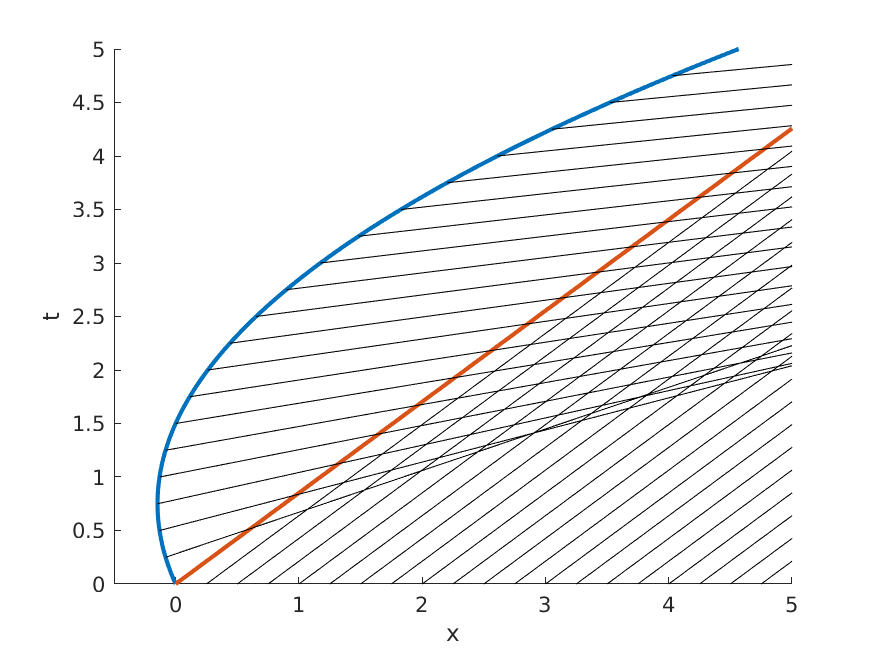
\includegraphics[width=40em]{as09fig1}
    \centering
\end{figure}

\end{document}
